\section{Results}
This section shows the results of the implementation described in section \cref{sec:implementation-details} and are obtained on the 1080 video with the convolution algorithm using the $H1$ matrix described in \cref{sec:methodology}. The machine used for the testing was provided with Intel(R) Xeon(R) Gold 5120 CPU @ 2.20GHz with 32 cores.

Let us first analyze the threads, then the different options tried with FastFlow, and finally a general comparison.

\begin{figure}[!htp]
    \centering
    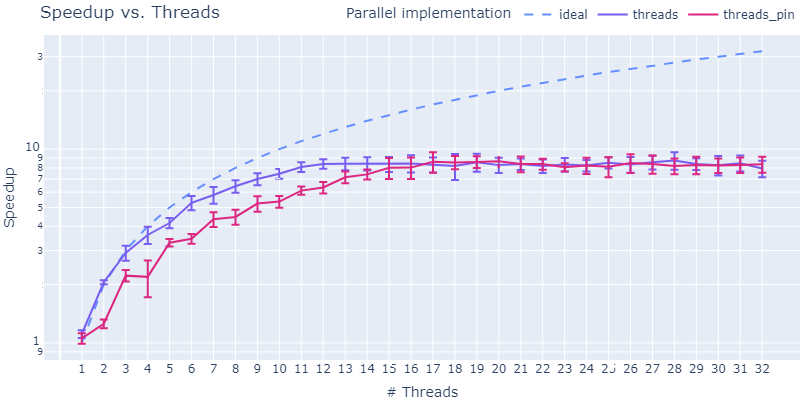
\includegraphics[width=\columnwidth]{1080_speedup_threads}
    \caption{Speedup of Threads vs Pinned threads with the convolution algorithm with H1 over a 1080p video.}
    \label{fig:1080-speedup-stream-threads}
\end{figure}
Regarding threads, two options were tried, namely with and without pinning on the 32 cores. In such a way as to be able to avoid the overhead of the context switch. As can be seen in \cref{fig:1080-speedup-stream-threads}, pinning does not go to improve speedup at all, in fact when the number of cores is low the situation gets worse. Here the explanation could be that setting affinity leads to making worse choices than the kernel would have made, but for a number of threads approaching the number of cores in the machine there begin to be slight and sporadic improvements.

\begin{figure}[!htp]
    \centering
    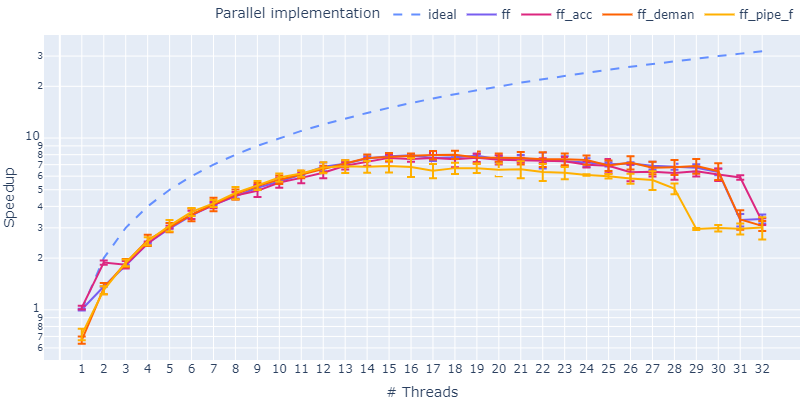
\includegraphics[width=\columnwidth]{1080_speedup_ff}
    \caption{Speedup of FastFlow with the convolution algorithm with H1 over a 1080p video.}
    \label{fig:1080-speedup-stream-ff}
\end{figure}
Turning instead to the implementation with FastFlow, the behaviors show subtle differences in \cref{fig:1080-speedup-stream-ff}. Analyzing \mintinline{bash}{ff} and \mintinline{bash}{ff_acc}, we see how the elimination of the collector in \mintinline{bash}{ff_acc} allows for one free thread to use and thus greater speedup when the machine cores are saturated. It therefore makes sense to avoid using a thread just to accumulate the number of frames with motion.
Considering instead \mintinline{bash}{ff} and \mintinline{bash}{ff_on_demand}, we see how the last one has only slightly better performance, but this was an expected behavior, due to the fact that motion detection computation presents for each frame a fairly homogeneous complexity, plus this scheduling makes sense when the emitter does not become the bottleneck, but this is not our case.
Finally, between the normal form \mintinline{bash}{ff} and the pipe with the farm \mintinline{bash}{ff_pipe}, it can be seen that the latter has slightly better behavior initially but then gets worse. The normal form is theoretically better, but it must be said that the steady state alternative has communication costs that are masked, at least until the bottleneck becomes the emitter. From that point on, the normal form begins to dominate.

\begin{figure}[!htp]
    \centering
    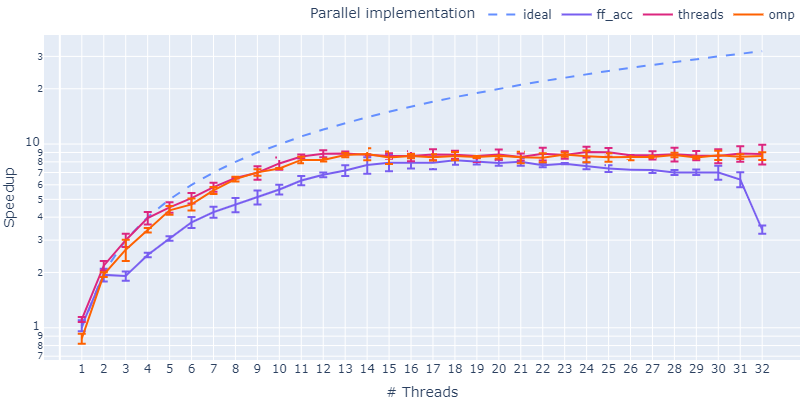
\includegraphics[width=\columnwidth]{1080_speedup_comparison}
    \caption{Speedup of Threads, FastFlow and OMP, with the convolution algorithm with H1 over a 1080p video.}
    \label{fig:1080-speedup-stream-comparison}
\end{figure}
To conclude, one can look at the speedup in \cref{fig:1080-speedup-stream-comparison} that reports the threads, \mintinline{bash}{ff_acc} and OMP. The implementation with threads remains almost always the best, but the gap between the first two is not as marked. Fast Flow has a slightly lower speedup with a low number of threads, but as the number of threads increases it recovers. There is a slight downward spike at the end that could be due to a context switch on the emitter that has become a bottleneck in that case. Moreover, by looking at the efficiency \cref{fig:1080-efficiency-stream-comparison} you can see that has dropped a lot, so throwing more threads at the problem, wouldn't help much.

As for the other kernels, the models have extremely similar behavior. For more details, you may refer to the attached code.

\begin{figure}[!htp]
    \centering
    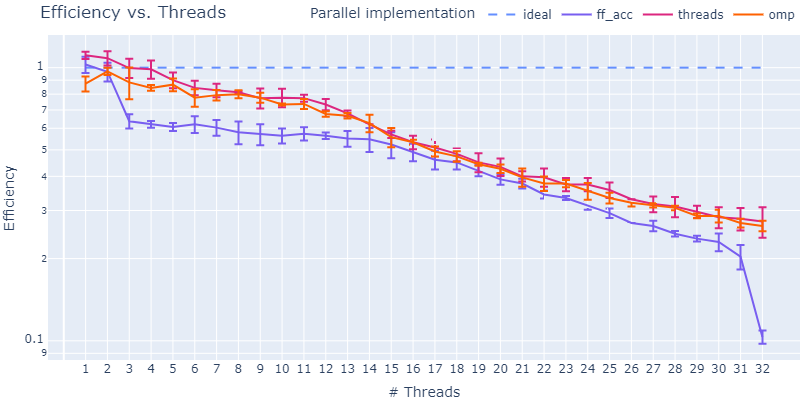
\includegraphics[width=\columnwidth]{1080_efficiency_comparison}
    \caption{Efficiency of Threads, FastFlow and OMP, with the convolution algorithm with H1 over a 1080p video.}
    \label{fig:1080-efficiency-stream-comparison}
\end{figure}

\begin{figure}[!htp]
    \centering
    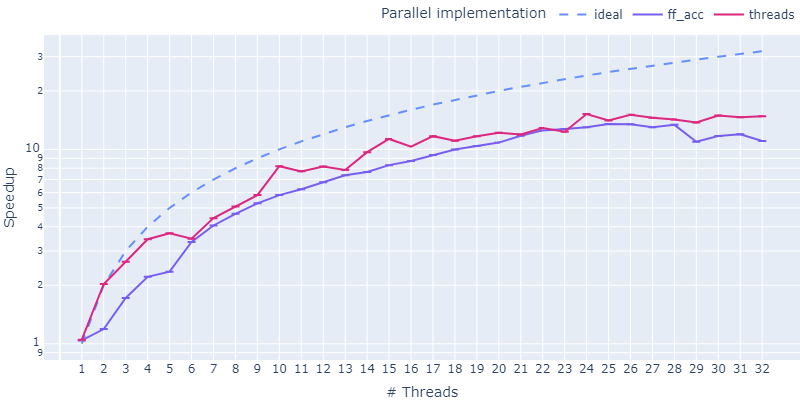
\includegraphics[width=\columnwidth]{1080_speedup_comparison_data}
    \caption{Speedup of Threads and FastFlow, with the convolution algorithm with H1 over a 1080p video that is preloaded in memory.}
    \label{fig:1080-speedup-data-comparison}
\end{figure}
Finally, in figure \cref{fig:1080-speedup-data-comparison}, there is the case where the entire video is first loaded into memory. Obviously, the speedup improves for all implementations, but this was also expected due to the fact that in \cref{sec:performance-model} we showed that the bottleneck is the I/O operation of the stream.

If we look at what was the estimated service time in the proposed performance model \cref{eq:service-time-estimated}, we can see that the theoretical lower bound was 7247$\mu s$. At this point, taking into consideration the best service times in obtained \cref{table:minimum-service-time}, we can see that we came very close. Obviously, there is some overhead that was not taken into account in the estimate, such as the time for concurrent access to the shared queue and the time to set up the whole parallel computation. 

\begin{table}[!h]
\centering
\begin{tabular}{lccc}
\hline
                       & Threads & Fast Flow & OMP     \\ \hline
Minimum Ts             & 7292.59 & 8092.39   & 7494.48 \\
Reached with \#threads & 24      & 18        & 14      \\ \hline
\end{tabular}
\caption{Minimum Service time $T_s$ achieved by the models with the numbers of threads needed.}
\label{table:minimum-service-time}
\end{table}